\documentclass[cs4size,a4paper,nofonts]{ctexart}
\usepackage[utf8]{inputenc}
\def\tjf{{\tt{田劲锋}}}
\def\titlec{Linux系统管理与维护(1):用户和用户群管理;软件包的管理}
\usepackage[a4paper,margin=2.2cm]{geometry} % 页面设置
\usepackage[unicode,breaklinks=true,
colorlinks=true,linkcolor=black,anchorcolor=black,citecolor=black,urlcolor=black,
pdftitle={\titlec},pdfauthor={\tjf}]{hyperref}
%\CTEXsetup[number=\chinese{section}, format={\large\sf\bfseries}]{section}
\usepackage{latexsym,amsmath,amssymb,bm}
\usepackage{graphicx}
\usepackage{subfigure}
\usepackage{wrapfig}
\usepackage{fancyvrb}
\DefineShortVerb{\|}
\fvset{frame=single}

\setmainfont{Times New Roman}
\setCJKmainfont[BoldFont={SimHei}]{SimSun}  % 主要字体:宋体、黑体
\setCJKsansfont[BoldFont={STZhongsong}]{STFangsong} % 次要字体:仿宋、中宋
\setCJKmonofont{KFKai} % 等宽字体:楷体

\CJKsetecglue{\hspace{0.1em}}
\renewcommand\CJKglue{\hskip -0.3pt plus 0.08\baselineskip}
\frenchspacing
\widowpenalty=10000
\linespread{1.2} % 行距

\usepackage[inline]{enumitem} % 调整列表样式
\setlist{noitemsep,align=left}
\setlist[itemize]{topsep=0pt,partopsep=0pt,itemsep=0pt,parsep=0pt}
\setlist[enumerate]{topsep=0pt,partopsep=0pt,itemsep=0pt,parsep=0pt}
\setlist[enumerate,1]{label={(\arabic*)}}
\setlist[enumerate,2]{label={\arabic*)}}

\CTEXsetup[beforeskip={0pt},afterskip={0pt}]{paragraph}

%\makeindex
\pagestyle{plain}

\begin{document}

%%%% 开始 %%%%

\begin{titlepage}

\begin{center}

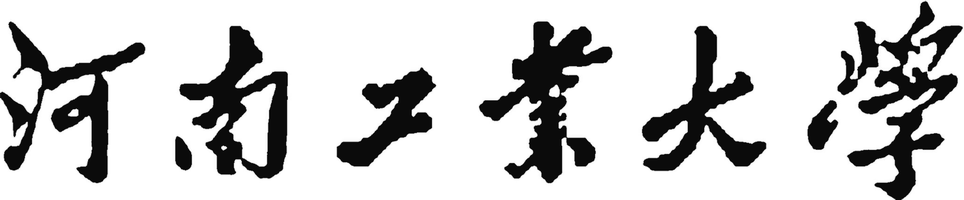
\includegraphics[height=1cm]{image/haut.png}

\vspace*{1cm}
{\liti\fontsize{48pt}{50pt}{课\quad 程\quad 设\quad 计}}

\vspace*{4cm}
{\fontsize{36}{80}\sf\bfseries \titlec}

\vspace*{1cm}
{\fontsize{30}{70}\sf\bfseries \titlee}

\vfill
{\large
\newcommand{\ctline}[2]{\makebox[6em][s]{\bf #1}:\underline{\makebox[14em][c]{\qquad #2\qquad}}\\}
\ctline{课程设计名称}{数据结构课程设计}
\ctline{专业班级}{计算机 1303 班}
\ctline{学生姓名}{\tjf}
\ctline{学号}{201316920311}
\ctline{指导教师}{白\quad 浩}
\ctline{课程设计时间}{\today}
}

\end{center}

\end{titlepage}


% \CTEXnoindent

\paragraph{实验题目:}\titlec

\paragraph{实验目的:}
(1)理解系统管理的各种配置文件;(2)掌握用户的添加、删除方法;(3)掌握组的添加、删除方法;(4)掌握软件包的管理工具的使用。

\paragraph{实验内容:}
\begin{enumerate}
\item 与用户账号有关的系统文件有哪些?使用cat命令查看这些文件并解释每一个文件中的各个字段所表示的含义是什么?
\item 与用户组有关的系统文件有哪些?使用cat命令查看这些文件并解释每一个文件中的各个字段所表示的含义是什么?
\item 分别用命令行的形式和图形化的形式添加用户newuser1和newuser2,然后用新用户登陆,看是否成功,然后用命令行的形式删除用户newuser2。
\item 分别用命令行的形式和图形化的形式添加用户组newgroup1和newgroup2,在组newgroup1加入用户newuser1。
\item 在Ubuntu系统下有哪些软件包的管理工具?
% \item 网络配置涉及哪些配置文件?查看其内容,并解释文件的基本内容。
% \item 如何使用命令配置一个网卡(IP地址、子网掩码、网管),如何使用命令挂载或卸载一个网卡?
\end{enumerate}

\paragraph{实验步骤:}

\newcommand{\image}[3][width=\textwidth]{
  \begin{minipage}[t]{0.5\textwidth}
    \centering
        \includegraphics[#1]{images/exp6/#2.png}
    \caption{#3}
    \label{fig:#3}
  \end{minipage}
}

\begin{enumerate}

\item 本地用户信息储存在|/etc/passwd|文件中。如图\ref{fig:用户文件},要查看系统上所有用户账户:
\begin{Verbatim}
$ cat /etc/passwd
\end{Verbatim}

一行代表一个用户,格式如下:
\begin{Verbatim}
account:password:UID:GID:GECOS:directory:shell
\end{Verbatim}

此处:
\begin{itemize}
\item |account|:用户名
\item |password|:用户密码
\item |UID|:用户的数字ID
\item |GID|:用户所在主组的数字ID
\item |GECOS|:可选的注释字段,通常记录用户全名
\item |directory|:用户的主目录({\tt\$HOME})
\item |shell|:用户的登陆shell(默认为|/bin/sh|)
\end{itemize}

现在的系统多使用影子密码。因为|passwd|文件对所有人可读,在里面存储密码(无论是否加密过)是很不安全的。在|password|字段,通常使用一个占位字符(|x|)代替。加密过的密码储存在|/etc/shadow|文件,如图\ref{fig:密码文件}和图\ref{fig:密码文件(尾部)},该文件对普通用户限制访问。

\begin{figure}[htp]
\image{1.passwd}{用户文件}
\image{2.shadow}{密码文件}
\end{figure}

\item |/etc/group|文件储存了系统中用户组的信息:
\begin{Verbatim}
$ cat /etc/group
\end{Verbatim}

如图\ref{fig:用户组文件},每行用冒号分开这些列:
\begin{itemize}
\item |group|:组名
\item |passwd|:组加密密码
\item |gid|:组的数ID
\item |member|:组的成员
\end{itemize}

如图\ref{fig:用户组密码},|/etc/gshadow|保存了组账号的安全信息如密码。

如图\ref{fig:超级用户组},|/etc/sudoers|表示可以运行sudo的用户。

\begin{figure}[htp]
\image{3.shadow}{密码文件(尾部)}
\image{4.group}{用户组文件}
\end{figure}

\begin{figure}[htp]
\image{5.gshadow}{用户组密码}
\image{6.sudoers}{超级用户组}
\end{figure}

\item 如图\ref{fig:建立用户1},建立用户1:
\begin{Verbatim}
$ sudo adduser newuser1
\end{Verbatim}

如图\ref{fig:登录用户1},登录用户1。

如图\ref{fig:用户账户}--\ref{fig:激活用户},使用图形化的方式建立用户2。

如图\ref{fig:登录用户2},登录用户2。

如图\ref{fig:删除用户2},删除用户2,并移除其主目录及其所有文件。
\begin{Verbatim}
$ sudo userdel -r newuser2
\end{Verbatim}

\begin{figure}[htp]
\image{7.newuser1}{建立用户1}
\image{12.login1}{登录用户1}
\end{figure}

\begin{figure}[htp]
\image{8.useracc}{用户账户}
\image{10.disabled}{默认禁用}
\end{figure}

\begin{figure}[htp]
\image{9.newuser2}{建立用户2}
\image{11.changepasswd}{激活用户}
\end{figure}

\begin{figure}[htp]
\image{13.login2}{登录用户2}
\image{14.userdel}{删除用户2}
\end{figure}

\item 如图\ref{fig:建立用户组},建立一个用户组:
\begin{Verbatim}
$ sudo groupadd newgroup1
\end{Verbatim}
然后将用户1加入该用户组。
\begin{Verbatim}
$ sudo gpasswd -a newuser1 newgroup1
\end{Verbatim}
这时候用|grep|再去查找用户组文件,就会发现用户1的身影了。

另外,Ubuntu并没有提供图形化的用户添加界面。

\begin{figure}[htp]
\image{15.newgroup1}{建立用户组}
\image{16.apthelp}{软件包管理器}
\end{figure}

\item Ubuntu继承Debian的体系,使用|apt-get|来安装管理软件包和解决依赖。如图\ref{fig:软件包管理器}显示了|apt-get|的帮助信息。

注意,学校机房由于使用了不再受到官方支持的旧非LTS版,所以需要另行配置成为新版本的软件源执行米安全的系统更新之后,才能够安装软件,比较浪费时间,不再演示。实际上大多数UNIX/Linux发行版都有他们自己的一套包管理器,而且成为程序员的必备工具。

\end{enumerate}

\paragraph{实验体会:}\quad

本次试验也相对比较容易,是关于用户组操作的的基本。用户组和多用户可以有效地利用一定的硬件资源,也为用户信息安全提供了保障。系统为了执行各种权限分配了很多不可登录的用户和用户组,这也是比较好的一个权限体系。

\end{document}
